\documentclass[fr]{../../../eplexercises}

\usepackage{../../../eplcode}
\usepackage{../../../eplunits}
\usepackage{float}
\usepackage[french,ruled,vlined]{algorithm2e}

\SetKwComment{Comment}{$\triangleright$\ }{}
\SetKw{KwBy}{by}

\graphicspath{{img/}}

\lstset{language=Java, basicstyle=\rm\small\ttfamily, tabsize=8}

\hypertitle[']{Algorithmique et structures de données}{5}{SINF}{1121}
{Gilles Peiffer}
{Pierre Schaus}

% TODO split exos up once solution can display "Solution à l'exercice x.x.x'"

\part{Types abstraits de données, complexité, collections \java{}; piles, files et listes liées}
\section{Exercices théoriques première partie}
\subsection*{Question 1.1.1}
Définissez ce qu'est un type abstrait de données
(\textsc{TAD}\footnote{\emph{Abstract data type} (\textsc{ADT}) en anglais}).
En \java{}, est-il préférable de décrire un TAD
par une classe ou une interface?
Pourquoi?

\begin{solution}
	Un \emph{type abstrait de données}
	est une spécification mathématique d'un ensemble de données
	et de l'ensemble des opérations
	que l'on peut effectuer sur elles.
	On qualifie d'abstrait ce type de données
	car il correspond à un cahier des charges
	qu'une structure de données doit implémenter.
	Sa représentation interne est inconnue de l'utilisateur.

	Il est préférable de décrire le type abstrait de données
	par une \emph{interface}.
	Une interface en \java{}
	est une liste de signatures de méthodes,
	sans implémentation.
	L'interface specifie le contrat pour le client,
	sans plus.
	De cette façon,
	l'implémentation est séparée,
	dans une toute autre classe.
	Un autre avantage des interfaces est
	que plusieurs représentations
	peuvent coexister dans un même programme.
	Ce n'est pas aussi simple
	lorsque l'\textsc{ADT} est représenté par une simple classe.
\end{solution}

\subsection*{Question 1.1.2}
Comment faire pour implémenter une \emph{pile}
par une liste simplement chaînée
où les opérations \lstinline|push| et \lstinline|pop|
se font en \textbf{fin de liste}?
Cette solution est-elle efficace? Argumentez.

\begin{solution}
	Une pile est caractérisée par son comportement \textsc{LIFO}.
	Pour \lstinline|push|,
	il faudrait d'abord itérer à travers la liste
	pour trouver le dernier élément.
	Ensuite, il faudrait
	attacher le nouveau n\oe{}ud derrière la liste
	en mettant une référence vers celui-ci
	dans le champ \lstinline|next| du dernier n\oe{}ud actuel,
	puis mettre le \lstinline|next|
	du nouveau n\oe{}ud à \lstinline|null|.
	En supposant que ces dernières opérations
	se fassent en temps constant,
	cette méthode serait donc en $\bigtheta(n)$,
	où $n$ est la taille de la liste,
	car il faut itérer sur tous les n\oe{}uds de la liste.
	Pour \lstinline|pop|,
	on se retrouve dans un cas similaire:
	il faut d'abord itérer jusqu'à l'avant-dernier n\oe{}ud,
	puis récupérer les données du dernier n\oe{}ud,
	et mettre la référence du nouveau dernier à \lstinline|null|.
	On a encore une fois une complexité en $\bigoh(n)$.
	Comme il est possible de faire ces opérations
	en temps constant ($\bigoh(1)$)
	en changeant la représentation interne de la stack,
	ce n'est pas une implémentation efficace.
\end{solution}

\subsection*{Question 1.1.3}
Quelles sont les implémentations possibles pour une pile?
En consultant la documentation sur l'\textsc{API} de \java{},
décrivez l'implémentation d'une pile par la classe
\lstinline|java.util.Stack|.
Allez voir le code source
de l'implémentation \lstinline|java.util.Stack|
(\texttt{ctrl+B} depuis IntelliJ).

Pourquoi pensez-vous que les développeurs de \java{}
ont choisi cette implémentation
(hint: argumentez au niveau de la mémoire et du garbage collector)?

\begin{solution}
	Il y a deux grandes manières d'implémenter une pile:
	avec des tableaux ou avec des listes chaînées.
	La pile est implémentée comme
	un \lstinline|Vector| d'un type générique,
	et a donc accès aux fonctions de la classe \lstinline|Vector|.
	La classe \lstinline|Stack|
	n'a que 6 méthodes:
	\lstinline|push()|, \lstinline|pop()|, \lstinline|peek()|,
	\lstinline|empty()|, \lstinline|search()| et un constructeur vide.

	Notamment pour la fonction \lstinline|pop|,
	on utilise une fonction de \lstinline|Vector|,
	\lstinline|removeElementAt()|,
	qui met la référence du n\oe{}ud devenu inutile
	à \lstinline|null|,
	de sorte à ce que le \textsc{GC}\footnote{Garbage collector.}
	puisse récupérer la mémoire.

	Une stack implémentée avec un tableau
	aurait comme complexités
	\begin{table}[H]
	\centering
	\begin{tabular}{ccc}
		\hline
		Opération & Liste chaînée & Tableau\\
		\lstinline|push| & $\bigoh(1)$ & $\bigoh(1)$ ou $\bigoh(n)$ (redimensionnement) \\
		\lstinline|pop| & $\bigoh(1)$ & $\bigoh(1)$ ou $\bigoh(n)$ (redimensionnement) \\
		$n$ \lstinline|push| & $\bigoh(n)$ & $\bigoh(n)$ (amorti) \\
		$n$ \lstinline|pop| & $\bigoh(n)$ & $\bigoh(n)$ (amorti) \\
		\hline
	\end{tabular}
	\end{table}
	Pour les complexités amorties,
	il suffit de remarquer que
	\[
	\sum_{i=1}^{\lg n} \frac{n}{2^i} < 2n \implies \bigoh(n)\,.
	\]
	\java{} utilise un tableau au lieu d'une liste chaînée
	pour diminuer le travail du \textsc{GC}.
	Quand on utilise une liste chaînée,
	les cas où on \lstinline|push| beaucoup
	font appel au \textsc{GC} trop souvent.
\end{solution}

\subsection*{Question 1.1.4}
Comment faire pour implémenter
le type abstrait de données \lstinline|Pile|
à l'aide de deux \emph{files}?
Décrivez en particulier le fonctionnement
des méthodes \lstinline|push| et \lstinline|pop| dans ce cas.

À titre d'exemple, précisez l'état de chacune des deux files
après avoir empilé les entiers \lstinline|1 2 3|
à partir d’une pile initialement vide.
Décrivez ce qu’il se passe ensuite
lorsque l’on effectue l’opération \lstinline|pop|.

Quelle est la complexité temporelle de ces méthodes
si l’on suppose
que chaque opération \lstinline|enqueue| et \lstinline|dequeue|
s’exécute en temps constant?

Cette implémentation d’une pile est-elle efficace
(pour $n$ opérations)
par rapport aux autres implémentations
présentées dans le livre de référence?

\nosolution

\subsection*{Question 1.1.5}
\begin{itemize}
	\item Qu'est-ce qu'un itérateur en \java{}
	(\lstinline|java.util.Iterator|)?
	\item Pourquoi est-ce util de définir une méthode
	\lstinline|iterator()| sur les structures de données?
	\item Que pensez-vous de permettre
	la modification d'une structure de données
	alors qu'on est en train d'itérer sur celle-ci?
\end{itemize}

Pour vous aider dans la réflexion,
nous vous invitons à lire la spécification de l'\textsc{API} \java{}
concernant la méthode \lstinline|remove()|.

Proposez une modification
du code de l’iterateur de \lstinline|Stack|
qui lance une erreur de type % had to add text so it breaks the line
\lstinline|java.util.ConcurrentModificationException|
si le client modifie la collection
avec un \lstinline|push()| ou \lstinline|pop()| durant l’itération.
Est-ce une bonne idée de laisser
l’implémentation de la méthode \lstinline|remove()| vide
si on ne désire pas permettre cette fonctionnalité?

\begin{solution}
	Un itérateur sert à passer à travers
	tous les éléments d'une collection.
	Il vaut mieux utiliser un itérateur que d'utiliser \lstinline|get()|
	car l'itérateur est plus intelligent
	et ne devra pas passer sur tous les n\oe{}uds de la collection
	avant d'arriver sur celui que l'on veut.
	Il ne faut absolument pas modifier la structure de données
	pendant qu'on itère dessus,
	à moins d'utiliser \lstinline|iterator.remove()|.
	On peut utiliser un compteur de \lstinline|push| et \lstinline|pop|
	pour voir si on a touché à la structure
	pendant que l'itérateur était dessus.
\end{solution}

\subsection*{Question 1.1.6}
La notation $\sim$ (tilde) est utilisée
dans le livre de référence
pour l'analyse des temps de calcul des algorithmes.
En quoi cette notation diffère ou ressemble
aux notations plus classiquement utilisées
$\bigoh$ (big Oh), $\bigomega$ (big Omega) et $\bigtheta$ (big Theta)?

Expliquez précisément les liens et similitudes entre celles-ci.
Que voyez-vous comme avantage à utiliser la notation $\sim$ (tilde)
plutôt que $\bigoh$ lorsque c'est possible?

\begin{solution}
	Ces notations sont similaires dans le sens où
	elles représentent la complexité algorithmique asymptotique.
	Cependant, dans le cas de la notation $\sim$
	on inclut un facteur multiplicatif de sorte à ce que
	\[
	g(N) \sim f(n) \textnormal{ signifie } \lim_{N \to \infty} \frac{g(N)}{f(N)} = 1\,.
	\]
	La notation $\sim$ est donc plus précise,
	et c'est pour cela qu'elle peut être préférable à la notation $\bigoh$.
\end{solution}

\subsection*{Question 1.1.7}
Expliquez comment nous pouvons
extraire la caractérisation $\sim$ (tilde)
de l'implémentation d'un algorithme
à l'aide du test \emph{Doubling ratio}.
\begin{itemize}
	\item Comment fonctionne ce test?
	\item Quelles sont les limites et avantages de ce test?
\end{itemize}
Supposons que nous mesurons les temps d'éxécution $T(n)$ suivants
(en secondes) d'un programme en fonction de la taille de l'entrée $n$:
\[
\begin{array}{cccccccc}
	\hline
	n & 1000 & 2000 & 4000 & 8000 & \num{16000} & \num{32000} & \num{64000} \\
	T(n) & 0 & 0 & 0.1 & 0.3 & 1.3 & 5.1 & 20.5 \\
	\hline
\end{array}
\]
\begin{itemize}
	\item Comment pouvez-vous caractériser au mieux
	l'ordre de croissance de cette fonction?
	\item Que serait le temps d'exécution pour $\num{128000}$?
\end{itemize}

\begin{solution}
	On se base sur la formule suivante:
	\[
	T(N) \sim a N^b \log N \iff T(2N) \sim a (2N)^b \log(2N)
	\]
	et donc
	\[
	\frac{T(2N)}{T(N)} \sim 2^b\,.
	\]
	Ce test n'est pas effectif si
	les ratios consécutifs n'approchent pas une valeur limite,
	mais pour la plupart des programmes,
	ils le font.
	Il a l'avantage d'être facile à effectuer,
	et qu'il fonctionne pour une grosse majorité des algorithmes.

	Pour ce qui en est des temps d'exécution proposés,
	on remarque que
	\[
	\frac{20.5}{5.1} \approx \frac{5.1}{1.3} \approx \frac{1.3}{0.3} \approx 4 \approx 2^b \implies b \approx 2\,.
	\]
	On a donc $T(n) \sim a n^2 \log n$. % exponent on log n?
	En multipliant le temps pour $\num{64000}$ par $4$,
	on peut prédire que le temps d'exécution
	sera d'environ $\SI{82}{\second}$ pour $n = \num{128000}$.
\end{solution}

\section{Exercices théoriques supplémentaires}

\subsection*{Question 1.1b.1}
Que signifient les paramètres \lstinline|-Xmx|, \lstinline|-Xms|
que l'on peut passer à la \textsc{JVM} pour l'exécution d'un bytecode?
Est-ce que ces paramètres peuvent influencer
la vitesse d'exécution d'un programme \java{}? Pourquoi?

\begin{solution}
	Le paramètre \lstinline|-Xmx| est
	une indication à la \textsc{JVM} de la taille maximale
	que peut atteindre le heap au cours de l'exécution du programme.
	Le paramètre \lstinline|-Xms| est
	une indication à la \textsc{JVM} de la taille initiale
	du heap au cours de l'exécution du programme.
	Il est possible d'améliorer la vitesse d'exécution
	en rendant les paramètres très grands,
	car alors le \textsc{GC} ne doit pas s'activer aussi souvent.
\end{solution}

\subsection*{Question 1.1b.2}
\begin{itemize}
	\item Qu’est-ce qu’un bon ensemble de tests unitaires
	pour vérifier l’exactitude d’une structure de données?
	\item Pensez-vous aux cas limites?
	\item Pensez-vous à
	la valeur maximale des entiers, doubles, etc.?
	\item En quoi la génération de données aléatoire
	peut être utile pour tester les structures de données?
	\item Pourquoi est-ce important
	de travailler avec une semence (seed) fixée?
	\item En quoi un outil d’analyse de couverture de code
	peut être utile
	(tel que \href{http://eclemma.org/jacoco/}{Jacoco})
	pour vous aider à concevoir des tests?
	\item Comment vérifier expérimentalement
	que l’implémentation d’une structure de données
	ou un algorithme a bien
	la complexité temporelle théorique attendue?
\end{itemize}

\nosolution

\part{Tri et propriétés des ensembles triés}
\section{Exercices théoriques première partie}
\subsection*{Question 2.1.1}
Étant donné un tableau contenant $n$ entiers triés,
et un nombre $x$ à insérer dans le tableau,
pouvez-vous indiquer un algorithme permettant
de trouver la position où insérer $x$
tout en gardant le tableau trié?

Quelle est la complexité de cet algorithme?

\begin{solution}
	L'algorithme par défaut pour faire ceci
	est l'algorithme du \emph{binary search},
	qui partitionne récursivement le tableau en deux.
	L'équation de récurrence que l'on résout est
	\[
	\left\{
	\begin{array}{rcl}
		f(n) & = & 1 + f\left(\frac{n}{2}\right)\,,\\
		f(0) & = & 1\,.
	\end{array}
	\right.
	\]
	Sa complexité est donc $\bigoh(\lg n)$,
	où $n$ est la taille du tableau.
\end{solution}

\subsection*{Question 2.1.2}
Nous considérons le problème très général où l’on a $n$ jobs
à accomplir pour des clients
et chaque job $j$ demande $t_j$ secondes pour l’accomplir.
Un seul job peut être effectué à la fois.

L’objectif est de terminer tous les jobs
tout en maximisant la satisfaction des clients.
Maximiser la satisfaction des clients revient à
construire un planning qui minimise le temps de complétion moyen des jobs.

Par exemple, si la durée des jobs est de $5, 8, 3, 4$
et que l’on effectue les jobs dans cet ordre,
les temps de fin seront de $5, 13, 16, 20$
et donc le temps de fin moyen sera de $\frac{5+13+16+20}{4} = 13.5$.
Prouvez (avec une preuve écrite!) que trier les $n$ jobs
dans l’ordre croissant des $t_j$ génère une solution optimale au problème.

\begin{solution}
	\begin{proof}
	On voit que le temps total $t$ est égal à
	\begin{align*}
	t &= \frac{t_1 + (t_1 + t_2) + \cdots + (t_1 + t_2 + \cdots + t_n)}{n}\\
	&= t_1 + \frac{n-1}{n} t_2 + \frac{n-2}{n} + \cdots + \frac{1}{n} t_n\\
	&= \sum_{i=1}^{n} \frac{n-i+1}{n} t_i\,.
	\end{align*}
	Par l'absurde.
	Soit une suite de jobs optimale telle que $t_a > t_b$.
	On voit que $2t_a + t_b > 2t_b + t_a$,
	et que donc si on ne trie pas les éléments,
	on aura un temps suboptimal\footnote{Enfin, suroptimal en fait\dots}.
	Il faut donc que
	\[
	t_1 \le t_2 \le t_3 \le \cdots \le t_n\,.
	\]
	\end{proof}
\end{solution}

\subsection*{Question 2.1.3}
Qu’entend-t-on par un algorithme de tri stable et en place (\emph{in place})?
Pour tout les algorithmes présentés dans le livre de référence,
indiquez s’ils sont en place (ou pas) ou stables (ou pas).

\begin{solution}
	Un algorithme est stable si il conserve l'ordre d'éléments
	dont la valeur est la même.
	Par exemple, on pourrait s'imaginer avoir une liste
	de nos \emph{followers} sur Twitter,
	triée par ordre alphabétique.
	Si on utilise un algorithme de tri stable
	pour les trier par nombre de tweets par exemple,
	ils seront toujours dans l'ordre alphabétique
	pour un même nombre de tweets.

	Un algorithme de tri est en place si il trie un tableau
	sans utiliser de structure de données auxiliaire.
	Cependant, un peu de mémoire supplémentaire est autorisée
	pour les variables auxiliaires.

	\begin{table}[H]
		\centering
		\begin{tabular}{ccc}
			algorithme & stable? & en place?\\
			\hline
			selection sort & non & oui\\
			insertion sort & oui & oui\\
			shellsort & non & oui\\
			quicksort & non & oui\\
			3-way quicksort & non & oui\\
			mergesort & oui & non\\
			heapsort & non & oui
		\end{tabular}
	\end{table}
\end{solution}

\subsection*{Question 2.1.4}
Comment trieriez-vous un tas de cartes
avec la restriction que les seules opérations permises sont:
\begin{enumerate}
	\item comparer les deux premières cartes;
	\item échanger les deux premières cartes;
	\item bouger la première carte à l’arrière du tas?
\end{enumerate}

\paragraph{Astuce} Le ``bubble sort'' est un algorithme de tri
qui consiste à comparer de manière répétée
les éléments consécutifs d’un tableau,
et à les permuter lorsqu’ils sont mal triés.
Cette opération est répétée jusqu’à ce que la liste soit triée.
Cet algorithme peut éventuellement vous inspirer.

\medskip
Écrivez le pseudocode de votre algorithme et donnez-en la complexité.

\begin{solution}
	Appelons la fonction de comparaison \lstinline|compareTo()|,
	avec la fonction \lstinline|toLast()|
	pour mettre la première carte à la fin
	et une fonction \lstinline|swap()|
	qui échange deux cartes (en l'occurrence, les deux premières).
	\begin{algorithm}[H]
	\DontPrintSemicolon
	\KwData{Un ensemble de $n$ cartes $\mathcal{C}$ sous forme de tableau.}
	\KwResult{Le même ensemble de cartes,
	trié dans l'ordre croissant selon la fonction de comparaison.}
	\Begin{
		\For{$os \gets 0$ \KwTo $n-1$ \KwBy $1$}{
			\For{$i \gets 0$ \KwTo $n - os - 1$ \KwBy $1$}{
				\If{$\mathcal{C}[0].\textnormal{compareTo}(\mathcal{C}[1]) > 0$)}{
					swap($\mathcal{C}[0]$, $\mathcal{C}[1]$)\;
				}
				toLast()\;
			}
			\For{$j \gets 0$ \KwTo $os - 1$ \KwBy $1$}{
				toLast()\;
			}
		}
	}
	\caption{Variante de bubble sort\label{algo:cardsort}}
\end{algorithm}
Cet algorithme\footnote{Baptisé \emph{cardsort} par l'auteur\dots}
a une complexité en $\bigoh(n^2)$.
\end{solution}

\subsection*{Question 2.1.5}
Comment trier une liste doublement chaînée
(qui ne permet donc pas d’accéder à une position par son indice) efficacement?
Quelle est la complexité de votre algorithme?

\begin{solution}
	On peut utiliser l'algorithme de mergesort,
	qui garde sa complexité en $\bigtheta(n \lg n)$ dans le pire cas.
	On peut également utiliser l'algorithme de quicksort.
\end{solution}

\subsection*{Question 2.1.6}
Imaginez un algorithme efficace
pour compter le nombre de paires de valeurs désordonnées.
Par exemple dans la séquence $1,3,2,5,6,4,8$
il y a les paires $(3,2),(5,4),(6,4)$ qui sont non ordonnées.
Justifiez la complexité de votre algorithme et donnez son pseudocode.

\paragraph{Astuce} Supposons deux tableaux $A$ et $B$,
soit $A.B$ le tableau résultat de la concaténation de $A$ et $B$.
Soit $\mathrm{nUnsorted}(A)$ le nombre de paires désordonnées
dans un tableau $A$.

Nous avons la propriété suivante que vous pouvez prouvez:
\[
\mathrm{nUnsorted}(A.B) = \mathrm{nUnsorted}(A) + \mathrm{nUnsorted}(B)
+ \abs{\{(i,j) \colon A[i] > B[j]\}}\,.
\]

Quelle est la complexité pour calculer $\abs{\{(i,j) \colon A[i] > B[j]\}}$?
Est-ce que cette complexité peut être améliorée si $A$ et $B$ sont triés?
Ne pouvez-vous pas calculer $\mathrm{nUnsorted}$ sur base d’une variante
d’un algorithme de tri bien connu qui s’exécute en $\bigoh(n \lg n)$?

\begin{solution}
	On peut utiliser une version légèrement modifiée de mergesort,
	où on détecte les inversions lors de l'opération de merge.
	Sa complexité est evidemment en $\bigtheta(n \lg n)$.
	Comme on le fait récursivement,
	on va ainsi compter toutes les inversions.

	\begin{algorithm}[H]
		\DontPrintSemicolon
		\KwData{Un tableau $l$ de $n$ nombres.}
		\KwResult{Le nombre de paires de nombres
		dans le mauvais ordre dans le tableau,
		ainsi que le tableau trié.}
		\Begin{
			\eIf{$\mathrm{len}(l) \le 1$}{
				\Return $(0, l)$\;
			}{
				mid $\gets$ $\mathrm{len}(l) / 2$\;
				cleft, $A$ $\gets$ mergesort($l$[0:mid])\;
				cright, $B$ $\gets$ mergesort($l$[mid:])\;
				cmerge, merged $\gets$ merge($A$, $B$)\;
				total $\gets$ cleft $+$ cright $+$ cmerge\;
				\Return total, merged\;
			}
		}
	\caption{Mergesort\label{algo:mergesort_inv}}
	\end{algorithm}
	\bigskip

	\begin{algorithm}[H]
		\DontPrintSemicolon
		\KwData{Deux parties d'un tableau, $A$ et $B$.}
		\KwResult{Le nombre de paires de nombres
		dans le mauvais ordre dans le tableau,
		ainsi que le tableau trié.}
		\Begin{
			li, ri $\gets$ 0, 0\;
			merged $\gets$ []\;
			count $\gets$ 0\;
			\While{li $< \mathrm{len}$($A$) and ri $< \mathrm{len}$($B$)}{
				\eIf{$A$[li] $< B$[ri]}{
					merged.append($A$[li])\;
					li $\gets$ li $+$ 1\;
				}{
					count $\gets$ count $+$ 1\;
					merged.append($B$[ri])\;
					ri $\gets$ ri $+$ 1\;
				}
			}
			\If{li $< \mathrm{len}$($A$)}{
				merged.extend($A$[li:])\;
			}
			\ElseIf{ri $< \mathrm{len}$($B$)}{
				merged.extend($B$[ri:])\;
			}
			\Return count, merged\;
		}
	\caption{Merge\label{algo:merge_inv}}
	\end{algorithm}
\end{solution}

\subsection*{Question 2.1.7}
Imaginons que nous souhaitons trier des objets \lstinline|Person|
de manière lexicographique par leur (poids, age, taille)
mais aussi des objets \lstinline|Student| par leur (age, note, année),
comment faire pour ne pas dupliquer l’algorithme de tri
spécifiquement pour ces classes?

Expliquez pourquoi les notions
de \lstinline|Comparable| et \lstinline|Comparator| de \java{}
sont utiles pour cela?
Expliquez comment vous implémenteriez un \lstinline|Comparator| efficace
pour des \lstinline|String|.

\begin{solution}
	Il faut que \lstinline|class Person implements Comparable<Person>|.
	On doit alors implémenter une fonction \lstinline|compareTo()|,
	qui est la fonction que \java{} appelle
	lorsqu'il essaie de trier des objets.
	L'algorithme de tri va utiliser
	la fonction \lstinline|compareTo()| propre
	au type d'objet qu'il essaie de trier.

	Comme en \java{}, il est impossible de faire
	\lstinline|class Student extends Person implements Comparable<Student>|,
	on utilise un \lstinline|Comparator|:
	\lstinline|class Person implements Comparator<Person>|.
\end{solution}

\subsection*{Question 2.1.8}
Est-il possible d’obtenir un tri stable
au départ d’un algorithme de tri non stable?
Comment?

\begin{solution}
	Oui; il suffit de soit trier d'abord sur un élément de l'objet
	puis sur un indice qu'on lui avait donné dans l'ordre initial,
	soit d'utiliser un dictionnaire\footnote{Plus tard dans le cours.}.
\end{solution}

\subsection*{Question 2.1.9}
Comment feriez-vous pour obtenir la 3\ieme{} plus petite valeur
dans un tableau d’un million de \lstinline|int|?
Quelle est la complexité de votre algorithme?

\begin{solution}
	On tient trois variables,
	et à chaque élément du tableau,
	on regarde si il fait partie des trois plus petits jusque là,
	et si oui, on le met dans sa position (1, 2 ou 3)
	et on réarrange les autres 2.
	Cet algorithme parcourt une fois la liste,
	et fait des opérations à temps constant.
	Il est donc $\bigoh(n)$.
\end{solution}

\subsection*{Question 2.1.10}
Comment feriez-vous pour obtenir la médiane
d’un tableau de valeurs (donc la $\frac{n}{2}$-ième valeur)?
Quelle est la complexité de votre algorithme?

\paragraph{Astuce} Que pouvez-vous déduire
concernant la position de la médiane
après l’opération de partitionnement autour d’une valeur $v$
dans l’algorithme \emph{quicksort}?

\begin{solution}
	On utilise l'algorithme quicksort,
	en prenant un pivot et en ne s'occupant que
	de la partie du tableau contenant la valeur médiane
	(c'est possible car pour quicksort,
	le pivot se retrouve toujours à sa place finale après un pivotement).
	L'algorithme est donc en $\bigoh(n \log n)$.
\end{solution}

\subsection*{Question 2.1.11}
\label{q:int_vs_integer}
Qu’est-ce que le Autoboxing and Unboxing en \java{}?
En quoi est-ce que cela peut impacter les performances d’un algorithme de tri?

Comparer les performance de \lstinline|java.util.Sort|
sur un tableau de \num{10000000} entrées composé de \lstinline|int|
et le même tableau avec des \lstinline|Integer|.

\begin{solution}
	L'\emph{autoboxing} est la conversion automatique que fait
	le compilateur \java{} entre les types primitifs
	et leurs classes Wrapper.

	L'\emph{unboxing} est la conversion inverse,
	c'est-à-dire celle que fait le compilateur \java{} entre
	les classes Wrapper et leurs types primitifs associés.

	Ces opérations prennent pas mal de temps,
	et il est donc conseillé
	d'utiliser le plus possible les types primitifs.
\end{solution}

\subsection*{Question 2.1.12}
Qu’est-ce qu’un \emph{profiler} de code?
Quelles informations fournies par un profiler
pourriez-vous utiliser pour améliorer les performances de vos algorithmes
et structures de données de manière générale (vitesse, mémoire, \textsc{GC})?

Un bon profiler gratuit est \href{https://visualvm.github.io}{VirtualVM}.

Utilisez \href{https://visualvm.github.io}{VirtualVM} sur votre code
pour la question~\ref{q:int_vs_integer}.

\begin{solution}
	Un \emph{profiler} de code est un logiciel qui permet
	de connaître le comportement d'un autre logiciel à l'exécution.
	Il permet de contrôler:
	\begin{itemize}
		\item la liste des fonctions appelées
		et le temps passé dans chacune d'elles;
		\item l'utilisation processeur;
		\item l'utilisation mémoire.
	\end{itemize}
	Il permet donc aussi de voir là où se trouvent les problèmes
	dans un code.
\end{solution}

\section{Exercices théoriques: deuxième partie}
\subsection*{Question 2.2.1}
Écrivez une méthode qui prend en entrée un tableau d’intervalles
et qui retourne l’union de ces intervalles
comme un tableau d’intervalles disjoints.
On considère que les intervalles d’input
sont donnés sous la forme de deux tableaux \lstinline|int[] min, int[] max;|
où le $i$\ieme{} intervalle
est donné par \lstinline|(min[i],max[i])|.
Exemple d’entrée: \lstinline|min=[5,0,1,6,2], max=[7,2,2,8,3]|
donnerait en sortie \lstinline|min=[0,5], max=[3,8]|.
Écrivez le pseudocode.
Quelle est la complexité de votre méthode?

\begin{solution}
	\begin{algorithm}[H]
		\DontPrintSemicolon
		\KwData{Deux tableaux d'entiers, }
		\KwResult{Le nombre minimal d'intervalles
		couvrant la même partie des réels.}
		\Begin{
			$S \gets (\texttt{min}[0],+1),(\texttt{max}[0]+1,-1),\ldots, (\texttt{min}[n-1],+1),(\texttt{max}[n-1]+1,-1),(+\infty,0)$\;
			sort($S$)\Comment*[r]{De façon croissante en `a',
			decroissante en `b'}

			start $\gets S[0].\min$\;
			overlap $\gets S[0].b$\Comment*[r]{Toujours $+1$}
			union $\gets \{\}$\;
			$i \gets 1$\;
			\While{$i < 2n$} {
				overlap $\gets$ overlap $+ S[i].b$\;
				\If(\Comment*[f]{Intervalle fermé}){overlap == $0$}{
				union.append([start..$S[i].a$])\;
					start $\gets S[i+1].a$\Comment*[r]{Pas un problème
					car on a un élément dummy en $2n$}
				}
				$i \gets i + 1$\;
			}
			\Return union
		}
	\caption{Union d'intervalles\label{algo:interval_union}}
	\end{algorithm}

	Cet algorithme est en $\bigoh(n \log n)$
	car on doit trier le tableau $S$.
\end{solution}

\subsection*{Question 2.2.2}
Vous devez trier un grand tableau
qui a pour propriété qu’il ne contient
que des valeurs dans l’ensemble $\{0,1,2\}$.
Quel algorithme de tri suggérez-vous?
Écrivez le code.
Quelle sera la complexité pour trier le tableau?
Discutez cette complexité
par rapport à la borne inférieure
d’un algorithme de tri (Proposition~1 pp. 280--281).

\begin{solution}
	Dans ce cas,
	il peut être utile d'utiliser l'algorithme \emph{counting sort}.
	Cet algorithme a une complexité en $\bigtheta(n+k)$,
	où $n$ est la taille du tableau en entrée
	et $k$ est l'élément le plus grand du tableau.
	Cet algorithme s'écrit comme suit:
	\lstinputlisting{code/CountingSort.java}

	Il est possible d'adapter cet algorithme
	dans le cas où $k$ est très grand mais où il n'y a que peu de valeurs.
	Cet algorithme peut tourner en temps linéaire
	malgré la proposition suivante:
	\begin{myprop}[Proposition~1 pp. 280--281]
		Aucun algorithme basé sur les comparaisons
		ne peut garantir trier $N$ objets
		en moins que $\sim N \lg N$ comparaisons.
	\end{myprop}
	On remarque ici qu'il ne s'agit pas
	d'un algorithme basé sur les comparaisons.

	Une autre possibilité
	est le \emph{quicksort with 3-way partitioning}\footnote{Qui est
	un peu plus difficile à implémenter\ldots}.
\end{solution}

\subsection*{Question 2.2.3}
Le mode d’un tableau de nombres
est le nombre qui apparait le plus fréquemment dans le tableau.
Par exemple $(4,6,2,4,3,1)$ a le mode $4$.
Donnez un algorithme efficace pour calculer le mode
d’un tableau de $n$ nombres.
Quid si on sait que le tableau ne contient que des valeurs de $0$ à $k$?

\begin{solution}
	Une solution basée sur les algorithmes de tri
	est de simplement appliquer un algorithme tel que \emph{quicksort}
	pour trier les éléments du tableau,
	puis ensuite de parcourir linéairement celui-ci
	pour trouver lequel des éléments apparaît le plus souvent.
	On a donc une complexité (sauf pour les cas pathologiques) en
	$\bigoh(n \log n)$.
	Dans le cas de quicksort, on peut gagner encore quelques opérations
	en ne calculant pas les appels récursifs
	ne pouvant pas livrer un nouveau meilleur mode.

	Si le tableau ne contient que des valeurs de $0$ à $k$,
	on peut alors utiliser un \emph{counting sort}
	de sorte\footnote{Hah!} à obtenir une compléxité en $\bigoh(n+k)$.

	On peut aussi noter que si on ne se limite pas aux algorithmes de tri,
	il y a moyen de faire ce calcul en temps linéaire
	en utilisant des tables de hachage.
\end{solution}

\subsection*{Question 2.2.4}
Étant donné deux ensembles $\mathcal{S}_1$ et $\mathcal{S}_2$
(chacun de taille $n$),
et un nombre $x$.
Décrivez un algorithme efficace pour trouver
s’il existe une paire $(a,b)$ avec $a \in \mathcal{S}_1, b \in \mathcal{S}_2$
telle que $a+b=x$.
Quelle est la complexité de votre algorithme?
Quid si les ensembles sont dans des tableaux déjà triés?

\begin{solution}
	En utilisant les algorithmes de tri,
	il faut $\bigoh(n \log n)$ pour trier un des tableaux ($a$),
	puis encore une fois $\bigoh(n \log n)$
	pour parcourir le tableau non trié ($b$)
	et de faire une recherche dichotomique
	sur $a$ pour trouver $b=x-a$.

	Si les tableaux sont déjà triés auparavant,
	on peut mettre des bornes plus fortes
	pour l'algorithme de binary search,
	mais on garde la même complexité.

	Notons que ce problème est une forme du problème 2SUM,
	pour lequel on a des algorithmes spécialisés tournant en $\bigoh(n)$.
\end{solution}

\subsection*{Question 2.2.5}
Même question que la précédente mais pour un seul ensemble.
Quid si l’ensemble est dans un tableau déjà trié?

\begin{solution}
	La réponse est la même que pour la question précédente.
\end{solution}

\subsection*{Question 2.2.6}
Donnez un algorithme pour calculer
l’union de deux ensembles $\mathcal{A}$ et $\mathcal{B}$.
Supposons dans un second temps,
que l’ensemble $\mathcal{A}$ déjà trié
a une taille $n$ et l’ensemble $\mathcal{B}$ également trié
a une taille $n^2$.
Quelle serait la complexité,
est-ce que votre algorithme change?

\begin{solution}
	Il y a plusieurs solutions
	(soit $\mathcal{A}$ de taille $n$ et $\mathcal{B}$ de taille $m$):
	\begin{enumerate}
		\item \label{item1} On met tout dans un grand tableau,
		et on trie celui-ci,
		puis on enlève les doublons.
		Cet algorithme prend donc $\bigoh((m+n) \log(m+n))$.
		\item \label{item2} On trie chaque ensemble séparément,
		puis on met tout ensemble en retirant les doublons.
		Cet algorithme prend $\bigoh(m \log m + n \log n)$.
		\item \label{item3} Supposons $m = n^2$.
		Pour chaque élément du petit,
		on fait une recherche dichotomique sur le grand
		pour savoir s'il faut rajouter cet élément dans l'union.
		Cette étape prend $\bigoh(2n \log n)$ et on a donc
		$\bigoh(n^2 + 2n \log n)$.
		Si on avait fait l'inverse,
		on aurait $\bigoh(n^2 \log n + n)$,
		ce qui est un peu moins bien.
		\begin{figure}[H]
		\centering
		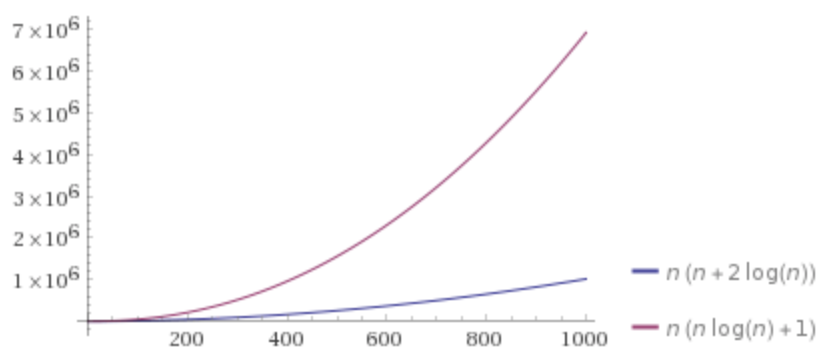
\includegraphics[width=0.5\textwidth]{algo_comp.png}
		\caption{Comparaison des algorithmes du point \ref{item3}.}
		\label{fig:algo_comp}
		\end{figure}
	\end{enumerate}

	Pour ce qui en est des complexités
	des points \ref{item1} et \ref{item2},
	elles sont égales si $m = n$.
\end{solution}

\subsection*{Question 2.2.7}
\label{q:line_column_sorted_array}
Étant donné une matrice de nombres entiers
qui sont triés le long des lignes et des colonnes,
comment trouver un nombre donné dans la matrice de manière efficace?
Indice: il existe un algorithme en temps $\bigoh(n+m)$
pour une matrice $n \times m$.
Pour cela commencez dans le coin supérieur droit
et comparez avec le nombre recherché.
Quelles parties de la matrice pouvez-vous élaguer
dans votre recherche en fonction du résultat?

\begin{solution}
	On commence dans ce coin,
	et on regarde si le nombre donné
	est plus grand ou plus petit que la position actuelle.
	S'il est plus grand,
	on descend à la ligne en-dessous,
	et s'il est plus petit,
	on avance d'une case vers la gauche.
	\begin{figure}[H]
	\centering
	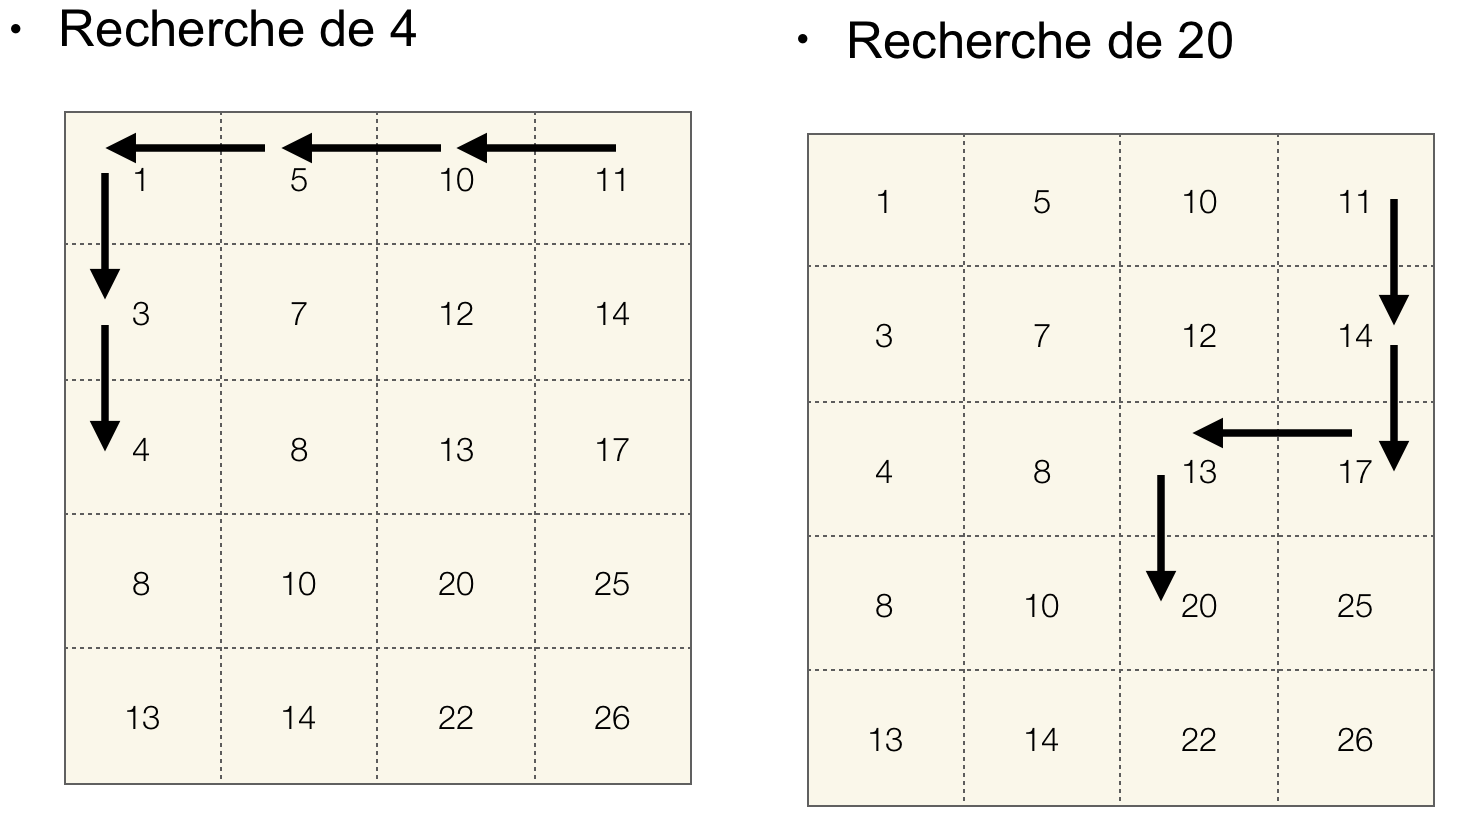
\includegraphics[width=\textwidth]{line_column_sorted_array.png}
	\caption{Réponse à la Question~2.2.7.}
	\label{fig:line_column_sorted_array}
	\end{figure}
	La \figuref{line_column_sorted_array}
	permet de visualiser cet algorithme.
\end{solution}

\end{document}
